\documentclass[a4paper,12pt]{article}

% Packages
\usepackage{graphicx}
\usepackage{amsmath}
\let\originaltimes\times
\renewcommand{\times}{\ensuremath{\originaltimes}}
\usepackage{geometry}
\usepackage{fancyhdr}
\usepackage{setspace}
\usepackage{titlesec}  % For title formatting
\usepackage{booktabs}
\usepackage[hidelinks]{hyperref}
\usepackage{float}
\usepackage[T1]{fontenc}
\usepackage{lmodern}
\usepackage{tikz}
\usetikzlibrary{positioning}
\graphicspath{{figures/}}
\setlength{\tabcolsep}{4pt}
\emergencystretch=2em

\geometry{margin=1in}
\setstretch{1.5}

% Header and Footer
\pagestyle{fancy}
\fancyhf{}
\fancyhead[L]{Comparative Data Mining Group Project}
\fancyhead[R]{\thepage}

% 标题格式
\titleformat{\section}{\normalfont\Large\bfseries}{\thesection}{1em}{}

% 封面页
\title{
    \vspace{2cm} % 保持图片间距不变
    \centering
    
\includegraphics[width=1\textwidth]{LU.jpg} \\ % 让图片居中，并调整大小
    \vspace{1cm} % 保持图片间距不变
    \textbf{\Huge Comparative Data Mining on German Credit and Thyroid Disease} \\
    \vspace{1cm} % 保持图片间距不变
    \large CDS535 - Data Mining \\
    \vspace{0.5cm} % 保持图片间距不变
    \large 2026
}
\author{
    \begin{minipage}{\textwidth}
        \centering
        Team name: Group 6 \\
        HU Zhongyuan (3162304) \\
        LING Tong (3162677) \\
        CHEN Yanwu (3162744) \\
        CHEN Yinan (3162550) \\
        ZHANG Yijie (3162641)
    \end{minipage} \\[25pt]
    \begin{minipage}{\textwidth}
        \centering
        \textbf{GitHub:} \url{https://github.com/chenyanwu83-blip/DM-Group-Project1}
    \end{minipage}
}
\date{}




\begin{document}

% Title Page
\maketitle
\thispagestyle{empty}
\newpage
\thispagestyle{empty}
\begin{abstract}
Class imbalance makes credit assessment and thyroid screening difficult to evaluate using accuracy alone. We compared decision trees, random forests, logistic regression and support vector classifiers on two UCI datasets. Each model was tested with plain training, SMOTE, class weighting and threshold adjustment. We used the same validation splits and fitted preprocessing within training folds. Apriori supplied association rules to help explain patterns in German Credit. Cost sensitive logistic regression achieved the highest mean F1 in the German Credit main experiment, while random forest with SMOTE led on sick. Strategies that improved recall could reduce precision, showing why accuracy alone can hide poor minority class performance. The additional ensemble study achieved a higher exploratory F1 on sick, but we did not directly test its advantage over the main experiment winner. Apriori found combinations associated with higher bad proportions and added to the tree model explanations. These results show that model choice depends on the dataset and decision objective. Independent validation is needed before practical use.

\newline

\noindent \textbf{Keywords}: classification, class imbalance, association rules, UCI datasets
\end{abstract}
\newpage
\thispagestyle{empty}
\tableofcontents
\thispagestyle{empty}
\newpage





% Table of Contents
% Start page numbering from the Table of Contents
\setcounter{page}{1}  % Start counting from 1

\section{Group Project Requirement}
\label{sec:requirement}

This group studies two datasets from the UCI Machine Learning Repository: Statlog German Credit Data and the sick subset of the Thyroid Disease collection~\cite{dua2019uci,uci_credit_g_1994,uci_thyroid_1986}. Each dataset follows a documented preprocessing, modeling, and evaluation workflow. The study includes four supervised algorithms, Apriori association rules, cross-validation, a locked holdout assessment, figures, and a reproducible comparison across models and datasets. An exploratory ensemble study is reported separately from the main experiment matrix.

The five members divide data preparation, modeling, evaluation, and report integration as shown in Table~\ref{tab:task-division}. The detailed contributions and approximate workload shares appear in the final appendix.

\begin{table}[htbp]
\centering
\small
\caption{Group 6 task division. The contribution appendix records the final individual workload shares.}
\label{tab:task-division}
\begin{tabular}{@{}p{0.20\linewidth}p{0.18\linewidth}p{0.52\linewidth}@{}}
\toprule
Member (ID) & Role & Main responsibility \\
\midrule
HU Zhongyuan (3162304) & A & credit-g audit, preprocessing, ensemble runs, and dataset writing \\
LING Tong (3162677) & B & sick audit, preprocessing, ensemble runs, and dataset writing \\
CHEN Yanwu (3162744) & C & Classifier pipelines, ensemble methods and tests, experiment runs, and method writing \\
CHEN Yinan (3162550) & D & Evaluation, figures, main and ensemble comparisons, and results writing \\
ZHANG Yijie (3162641) & E & Apriori analysis, report integration, references, and presentation coordination \\
\bottomrule
\end{tabular}
\end{table}


\section{Introduction}
\label{sec:introduction}

\subsection{Background and Motivation}
Automated credit scoring supports lending decisions in which the two error types are
economically asymmetric: approving an applicant who turns out to default (a missed
\texttt{bad} case) destroys principal, whereas rejecting a creditworthy applicant (a
false \texttt{bad} alarm) merely forgoes interest income. The Statlog German Credit
data makes this asymmetry explicit through an official 5:1 misclassification-cost
matrix, in which missing a \texttt{bad} applicant costs five times as much as
rejecting a \texttt{good} one~\cite{uci_credit_g_1994}. Class imbalance amplifies the
problem: \texttt{bad} applicants form only 30\% of \texttt{credit-g} and about 6\% of
the \texttt{sick} thyroid subset~\cite{uci_thyroid_1986}, so accuracy is dominated by
the majority class --- a trivial rule that always predicts \texttt{good} already
achieves 0.70 accuracy on \texttt{credit-g} while never identifying a single default.
Practitioners can draw on three families of remedies --- synthetic minority
over-sampling~\cite{chawla2002smote}, cost-sensitive training, and decision-threshold
adjustment --- yet their relative merits change with the model family and the degree
of imbalance, and are rarely compared under one leakage-safe protocol with an
application-grounded cost measure.

\subsection{Research Significance}
This project delivers such a comparison on two UCI datasets~\cite{dua2019uci} that
differ deliberately in scale, imbalance ratio, missingness and domain. For risk
management, it shows which imbalance intervention actually minimises the official
misclassification cost rather than a surrogate metric. For methodology, it
demonstrates a reproducible experimental discipline: preprocessing specifications
frozen before the main matrix, locked data splits, SHA-256 provenance chained from
raw data to every result file, and all imputation, encoding, scaling and resampling
fitted strictly inside the cross-validation folds, so that any observed gain is
attributable to the strategies rather than to information leakage. For
interpretability, association rules mined from the same data are triangulated
against tree-based model explanations. The full pipeline is implemented with
scikit-learn~\cite{pedregosa2011sklearn}, imbalanced-learn~\cite{lemaitre2017imblearn}
and mlxtend~\cite{raschka2018mlxtend}, with Weka~\cite{frank2016weka} as the course
reference tool.

\subsection{Research Questions and Contributions}
The study is organised around four research questions:
\begin{itemize}
  \item \textbf{RQ1.} Under class imbalance and asymmetric misclassification
  costs, how should the four candidate strategies (plain, SMOTE,
  cost-sensitive, threshold moving) and four model families be selected?
  The two datasets provide contrasting endpoints (clean/2.3:1 vs.\
  noisy/15.3:1), and the official 5:1 cost matrix is folded into this
  question as a first-class constraint.
  \item \textbf{RQ2.} Under what conditions does accuracy mislead model
  selection on imbalanced data, and which metrics (positive-class
  recall/F1, ROC-AUC, official misclassification cost) should drive
  evaluation and decision-making instead?
  \item \textbf{RQ3.} How do mixed attributes jointly determine feature
  treatment and model selection --- which features matter, and how should
  nominal attributes be encoded (one-hot vs.\ ordinal) for each model
  family (linear/kernel vs.\ tree-based)?
  \item \textbf{RQ4.} Do the learnt models make reliable decisions on new,
  unseen examples, as measured once on the locked hold-out sets of 300
  credit applicants and 1{,}132 patients?
\end{itemize}

\noindent The main contributions are: (i) a paired two-dataset design contrasting
five dimensions at once --- scale (1{,}000 vs.\ 3{,}772 records), imbalance (70:30
vs.\ 94:6), missingness (0 vs.\ 29.9\% of rows), attribute composition and domain ---
which directly probes RQ1; (ii) a full experiment matrix of four classifiers
(decision tree, random forest, logistic regression, RBF-SVM) $\times$ four
strategies (plain, SMOTE, cost-sensitive, threshold adjustment) built on
leakage-safe pipelines with locked splits; (iii) the official cost matrix treated
as a first-class evaluation axis alongside F1 and ROC-AUC (RQ2, RQ3); (iv) a
controlled encoding ablation with a supplementary attribution control that
separates encoding from scaling effects (RQ3); and (v) an interpretability
triangulation of Apriori rules, decision-tree paths and random-forest feature
importances (Section~\ref{sec:apriori}). Statistical comparisons use fold-level
tests with the Nadeau--Bengio
correction~\cite{nadeau2003inference,demsar2006comparison}. Experimental results
are reported in Section~\ref{sec:results}.

\section{Data Distribution and Preprocessing}
\label{sec:data}
\subsection{Statlog German Credit Data}

\textbf{Provenance and licence.} We use the Statlog German Credit data
(\texttt{credit-g})~\cite{uci_credit_g_1994}, donated by Hans Hofmann (University of
Hamburg, 1994) to the UCI Machine Learning Repository~\cite{dua2019uci} (UCI ID~144,
DOI 10.24432/C5NC77). The dataset is released under the CC BY 4.0 licence and is
cited accordingly.

\textbf{Attribute schema.} The dataset contains 1{,}000 applicants $\times$ 21
columns: 13 nominal attributes, 7 numeric attributes and the binary target
\texttt{class} (\texttt{good} vs.\ \texttt{bad}; the positive class is \texttt{bad}
throughout this report). The full 21-row dictionary with business semantics, value
sets and per-column missing counts is archived as
\texttt{results/credit-g\_schema.xlsx}.

\textbf{Class distribution and data quality.} Figure~\ref{fig:a_class} shows the
class distribution: 700 \texttt{good} versus 300 \texttt{bad}, i.e., a 30\%
positive rate and a moderate 70:30 imbalance. A systematic quality audit reports
zero missing values and zero duplicated rows across all 21 columns, so
\texttt{credit-g} requires no imputation and no row or column deletion. The 70:30
ratio also fixes the reference points used later: a majority-class baseline already
scores 0.70 accuracy (revisited in Section~\ref{sec:results}), and all resampling
and cost-sensitive strategies are motivated by this imbalance.

% Source: figures/fig_a_class.png = figures/fig1_class_distribution.png (src/a4_creditg_eda.py)
\begin{figure}[H]
\centering
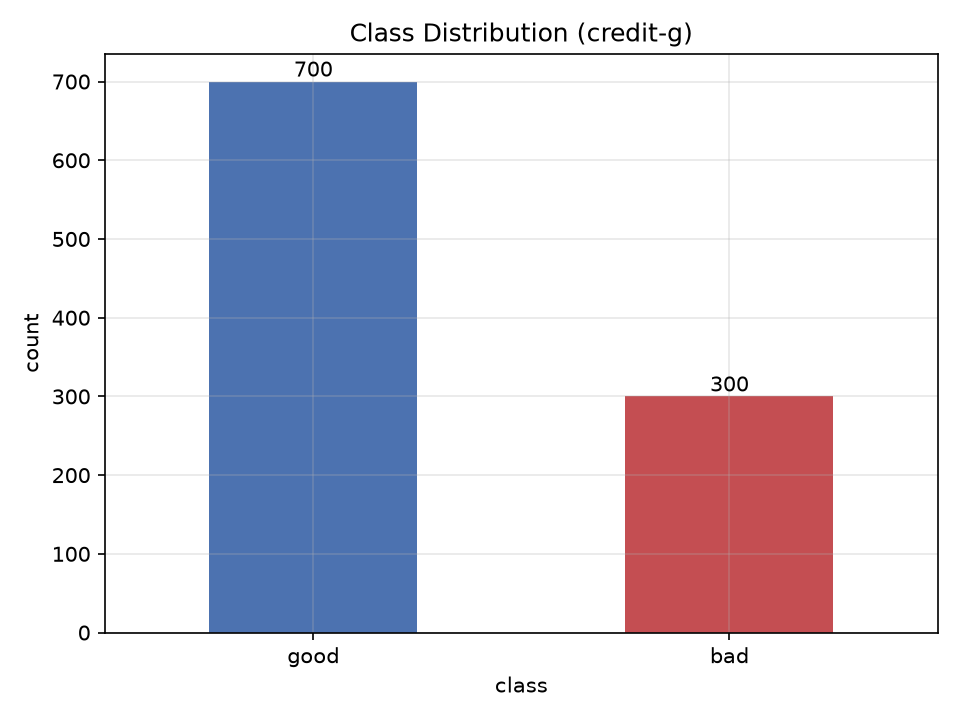
\includegraphics[width=0.55\textwidth]{figures/fig_a_class.png}
\caption{Class distribution of \texttt{credit-g} (1{,}000 records; positive class
= \texttt{bad}): 700 \texttt{good} vs.\ 300 \texttt{bad} (30\% positive rate), a
70:30 class imbalance. Source: \texttt{figures/fig1\_class\_distribution.png}
(\texttt{src/a4\_creditg\_eda.py}).}
\label{fig:a_class}
\end{figure}

\textbf{Descriptive statistics.} Of the seven numeric attributes, three are
genuinely continuous (\texttt{duration}, \texttt{credit\_amount}, \texttt{age}) and
four are ordinal grade fields on 1--4 or 1--2 scales. Figure~\ref{fig:a_numeric}
shows that all three continuous attributes are right-skewed --- for
\texttt{credit\_amount} the median (2{,}320 DM) lies far below the mean (3{,}271 DM)
and the maximum (18{,}424 DM) --- a skew that directly informs the discretisation
choice below.

% Source: figures/fig_a_numeric.png = figures/fig3_numeric_hist.png (src/a4_creditg_eda.py)
\begin{figure}[H]
\centering
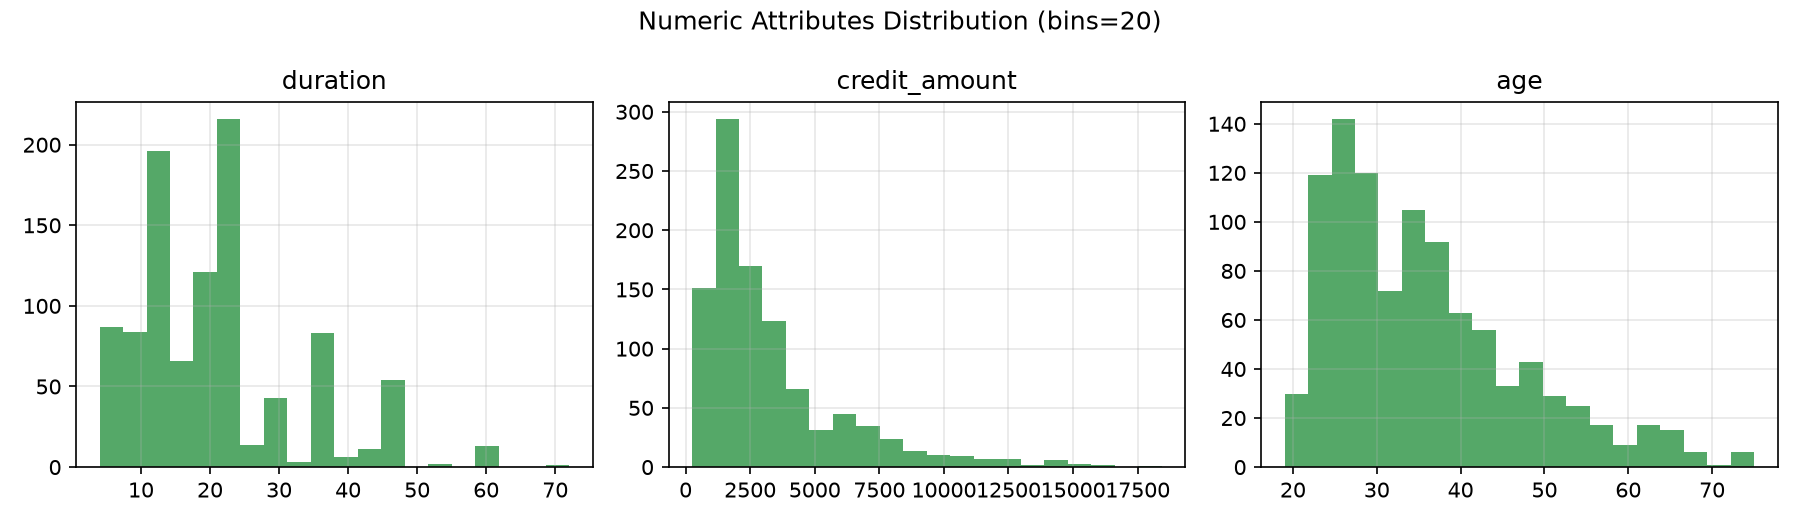
\includegraphics[width=0.95\textwidth]{figures/fig_a_numeric.png}
\caption{Histograms (bins = 20) of \texttt{duration}, \texttt{credit\_amount} and
\texttt{age} in \texttt{credit-g}; all three are right-skewed, with
\texttt{credit\_amount} ranging from 250 to 18{,}424 DM. Source:
\texttt{figures/fig3\_numeric\_hist.png} (\texttt{src/a4\_creditg\_eda.py}).}
\label{fig:a_numeric}
\end{figure}

Among the nominal attributes, \texttt{checking\_status} shows the clearest
relationship with the target. Figure~\ref{fig:a_checking} sorts its four values by
default rate: the \texttt{bad} share falls monotonically from 49.3\% (overdrawn
accounts, \texttt{<0}, 135 of 274) to 39.0\% (\texttt{0<=X<200}), 22.2\%
(\texttt{>=200}) and 11.7\% (no checking account, 46 of 394), straddling the 30\%
overall rate. This gradient is consistent with domain intuition (weaker account
standing, higher default risk) and is later corroborated by tree-based feature
importances in the interpretability analysis.

% Source: figures/fig_a_checking.png = figures/fig2_checking_status_class.png (src/a4_creditg_eda.py)
\begin{figure}[H]
\centering
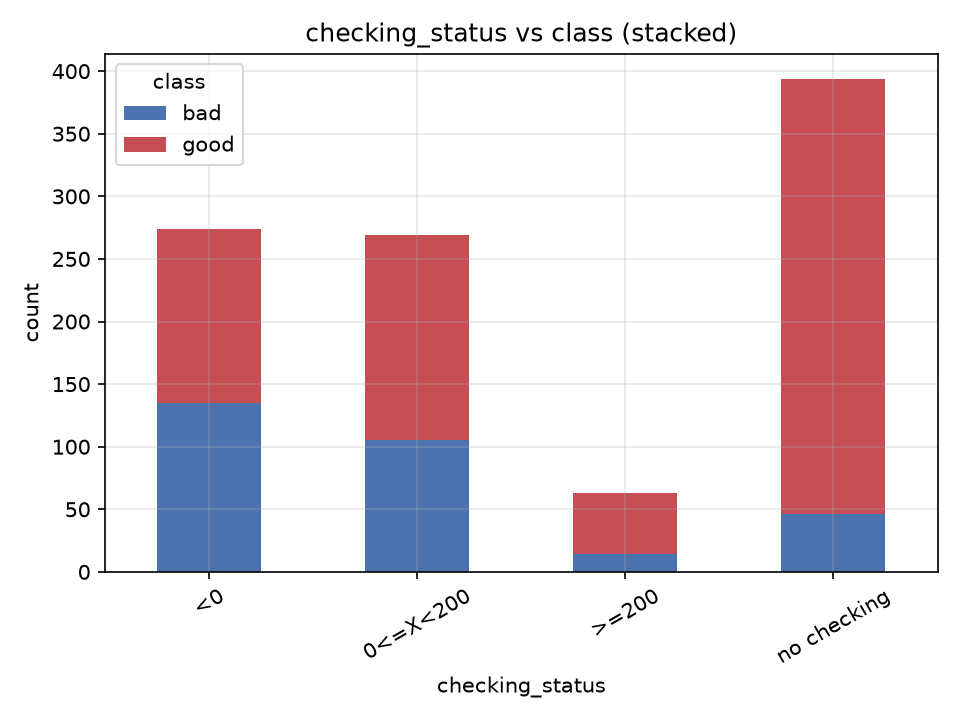
\includegraphics[width=0.72\textwidth]{figures/fig_a_checking.png}
\caption{Stacked class distribution by \texttt{checking\_status} in \texttt{credit-g},
sorted by default rate (positive class = \texttt{bad}). Overdrawn accounts
(\texttt{<0}) show the highest \texttt{bad} rate (49.3\%), accounts without a
checking account the lowest (11.7\%). Source:
\texttt{figures/fig2\_checking\_status\_class.png}
(\texttt{src/a4\_creditg\_eda.py}).}
\label{fig:a_checking}
\end{figure}

\textbf{Preprocessing decisions.} Four preprocessing decisions are adopted for
\texttt{credit-g}:
\begin{enumerate}
  \item \emph{No cleaning.} The quality audit (0 missing, 0 duplicated) removes the
  need for imputation or deletion; the raw table enters the pipelines unchanged.
  \item \emph{Linear and kernel models} (logistic regression, RBF-SVM) receive the
  13 nominal attributes one-hot encoded (\texttt{handle\_unknown='ignore'}) and the
  numeric attributes standardised to zero mean and unit variance.
  \item \emph{Tree-based models} (decision tree, random forest) receive ordinal
  codes for the nominal attributes (\texttt{unknown} $\rightarrow$ $-1$) and
  unscaled numerics: tree splits depend on orderings and thresholds only, so
  one-hot expansion would merely dilute split gains and scaling has no effect.
  \item \emph{Discretisation for association analysis}: the continuous attributes
  \texttt{duration}, \texttt{credit\_amount} and \texttt{age} are binned with
  \texttt{KBinsDiscretizer} into five \emph{quantile} bins, and nominal values are
  used as items directly (Section~\ref{sec:apriori}). Quantile bins rather than
  equal-width bins are used precisely because the right skew of
  Figure~\ref{fig:a_numeric} would collapse most records into the lowest equal-width
  bin.
\end{enumerate}

A controlled ablation confirms the branch assignment of decisions 2 and 3 (RQ3).
Table~\ref{tab:a_encoding} compares logistic regression under the two encodings by
stratified 10-fold cross-validation (seed 42; positive class \texttt{bad}): one-hot
encoding with standardised numerics outperforms ordinal encoding with raw numerics
on every metric, and the gains in F1 and ROC-AUC are statistically significant
under fold-level paired $t$-tests ($n = 10$, uncorrected). One-hot encoding with
standardised numerics is therefore used for all linear/kernel models and ordinal
codes with raw numerics for all tree-based models throughout the main matrix. Full
fold-level results are archived in \texttt{results/a6\_onehot\_comparison.csv} and
\texttt{results/a6\_onehot\_folds.csv}.

\begin{table}[H]
\centering
\caption{Encoding ablation on \texttt{credit-g} (logistic regression, stratified
10-fold CV, seed 42, positive class = \texttt{bad}; means over $n = 10$ folds).
Source: \texttt{results/a6\_onehot\_comparison.csv}.}
\label{tab:a_encoding}
\begin{tabular}{lrrrr}
\toprule
Encoding & Features & Accuracy & F1 (\texttt{bad}) & ROC-AUC \\
\midrule
One-hot + standardised numerics & 61 & \textbf{0.752} & \textbf{0.531} & \textbf{0.785} \\
Ordinal + raw numerics & 20 & 0.718 & 0.406 & 0.738 \\
\midrule
Paired $t$-test $p$ ($n = 10$ folds) & --- & 0.101 & 0.021 & 0.008 \\
\bottomrule
\end{tabular}
\end{table}

\subsection{Sick Dataset}
\label{sec:sick-data}
% B owns this subsection: UCI provenance, label meaning, missingness, and preprocessing.

The \textit{sick} dataset belongs to the UCI Thyroid Disease repository
(ID 102, DOI 10.24432/C5D010), with original data donated by the Garavan
Institute (1986) and redistributed under CC BY 4.0; we use the Weka-packed
variant (accepted by the course brief). The ``7,200 instances / 5
features'' on the UCI landing page describes the whole thyroid
repository, not this subset. The actual dataset contains
\textbf{3,772 instances $\times$ 30 attributes} (23 nominal, 7 numeric,
including the class). The class is severely imbalanced: 3,541
\textit{negative} versus 231 \textit{sick-euthyroid}, i.e.\ 6.1\%
positives (94:6); we treat \textit{sick} as the positive class
throughout. Two semantic notes we keep strict in wording:
\textit{sick-euthyroid} denotes a euthyroid patient whose
thyroid-related blood tests are abnormal --- notably low T3 --- while the
thyroid gland itself is not diseased; the pattern usually reflects severe
non-thyroidal illness such as chronic renal failure, diabetes or anaemia
(UCI \texttt{thyroid.theory}). It is \emph{not} hypothyroidism, which is a
separate sub-dataset. \textit{negative} means no thyroid abnormality
detected in this screening, not ``perfectly healthy''. 61
duplicate rows exist in the official distribution; we keep them to remain
consistent with the official instance count and disclose them as a
data-quality issue.

\subsubsection{Missing-value audit}
In total 6,064 cells (5.4\%) are missing, coded as ``?''. The audit
revealed a clean \emph{measurement mechanism}: every laboratory test
appears as a pair --- a \texttt{*\_measured} flag and the value itself ---
and whenever the flag reads \texttt{f} (test not performed), the paired
value is missing \emph{by design}. Across all six lab pairs the
consistency check found \textbf{zero anomalies}: the data is incomplete
but internally consistent. The extreme case is \textbf{TBG, 100\% missing
in all 3,772 rows} (its flag reads \texttt{f} in every row). After
removing TBG and its constant flag, 1,129 rows
(29.9\%) still carry at least one missing value
(Figs.~\ref{fig:sick-dist}--\ref{fig:sick-missing}).

\subsubsection{Handling decisions}
Three decisions follow directly from the audit, in the same
decision-plus-ablation style as the credit-g preprocessing above:

\begin{enumerate}
\item \textbf{Remove} TBG and its constant flag. A column with zero
observations cannot be imputed without fabricating data; column removal
involves no statistics and is leakage-free.
\item \textbf{Impute} the remaining columns \emph{inside} the imblearn
pipeline (numeric by mean, nominal by mode), so imputation statistics
are fitted on training folds only, alongside encoding, scaling and
SMOTE.
\item \textbf{Keep} the 61 duplicate rows, staying consistent with the
official instance count (disclosed above as a data-quality note).
\end{enumerate}

Decision~2 was validated by the same style of controlled ablation as the
credit-g encoding choice (Table~\ref{tab:a_encoding}): one decision
tree, one locked protocol, three missing-value treatments
(Table~\ref{tab:b_imputation}). Dropping incomplete rows discards
1{,}129 patients --- 19 of them positive --- for an F1 difference within
one standard deviation and the lowest AUC, and the two cohorts are not
even the same patients. Treating ``missing'' as its own category (an
option here because scikit-learn trees, unlike Weka's J48, reject
\texttt{NaN} values) performs no better. Fold-internal imputation keeps
all 3{,}772 instances and attains the best AUC, and was therefore locked
in the preprocessing spec (full fold-level results archived in
\texttt{results/b4\_missing\_comparison.csv}). The contrast with
credit-g is instructive: there the ablation \emph{changed} the decision
(which encoding to use), whereas here it \emph{confirmed} the default
--- the informative question on sick is not which treatment wins on F1,
but what deleting rows would cost.

\begin{table}[htbp]
\centering
\caption{Missing-value treatments on sick (decision tree, entropy,
\texttt{ccp\_alpha}=0.01; cv10, mean$\pm$std, ddof$=0$; positive
= sick-euthyroid).}
\label{tab:b_imputation}
\begin{tabular}{lccc}
\toprule
Treatment & Rows & F1 & ROC-AUC \\
\midrule
Fold-internal imputation (adopted) & 3{,}772 & 0.830$\pm$0.049 & \textbf{0.974} \\
Drop incomplete rows & 2{,}643 & 0.843$\pm$0.069 & 0.964 \\
``Missing'' as explicit category & 3{,}772 & 0.828$\pm$0.044 & 0.965 \\
\bottomrule
\end{tabular}
\end{table}
Finally, among the four base classifiers the random forest is the only
one whose precision is preserved under SMOTE (0.94$\to$0.91, vs.\
0.95$\to$0.60 for a single tree); Section~\ref{sec:results} sharpens this
account with the ensemble study, where AdaBoost shares the property and
plain bagging does not.

\begin{figure}[htbp]
\centering
\begin{minipage}{0.48\linewidth}
  \centering
  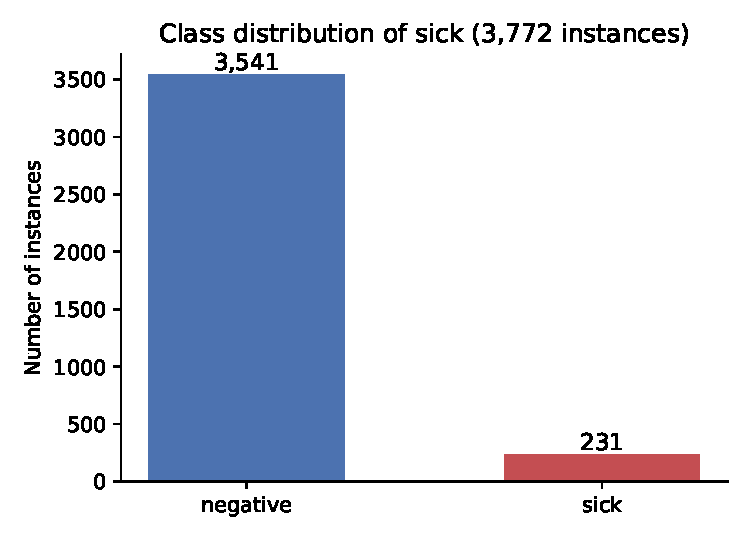
\includegraphics[width=\linewidth]{figures/fig_b_class.pdf}
  \caption{Class distribution of sick (3,541:231, 6.1\% positives; cv10,
  positive = sick-euthyroid).}\label{fig:sick-dist}
\end{minipage}\hfill
\begin{minipage}{0.48\linewidth}
  \centering
  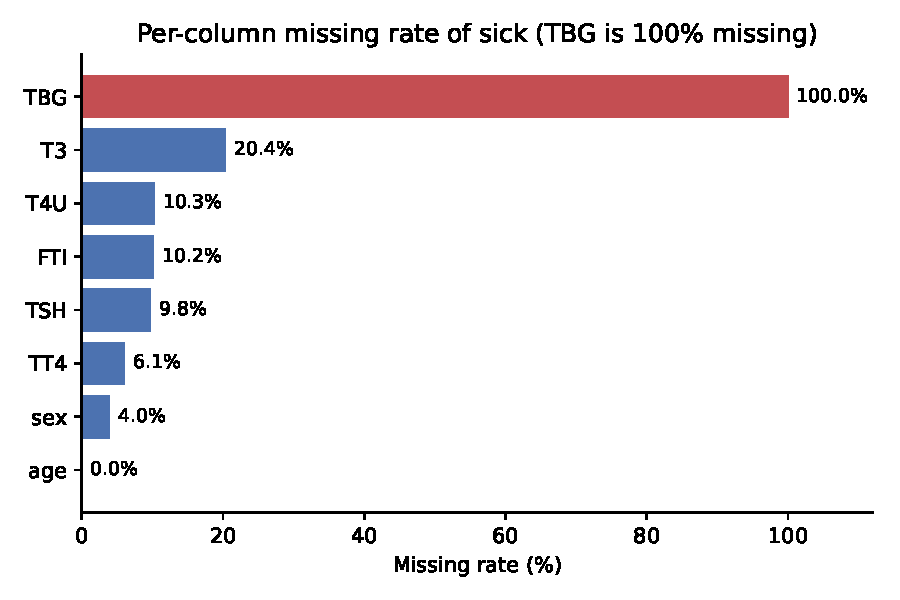
\includegraphics[width=\linewidth]{figures/fig_b_missing.pdf}
  \caption{Per-column missing rate of sick; TBG (red) is 100\% missing
  and removed rather than imputed.}\label{fig:sick-missing}
\end{minipage}
\end{figure}

\begin{figure}[htbp]
\centering
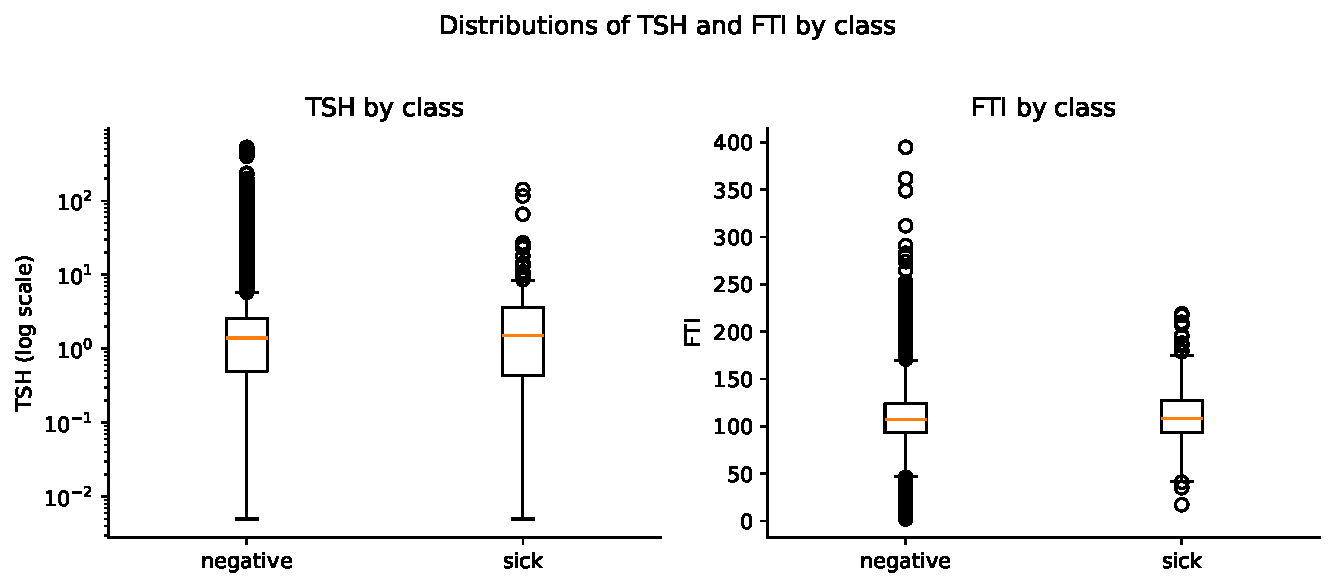
\includegraphics[width=0.62\linewidth]{figures/fig_b_box.pdf}
\caption{TSH (log scale) and FTI by class (raw data): heavy class overlap
(median TSH 1.4 vs.\ 1.5; FTI 107 vs.\ 108) shows no single lab value
separates the classes, motivating multivariate models.}\label{fig:sick-box}
\end{figure}

\section{Basic Concepts of Algorithms}
\label{sec:algorithms}

Our main matrix combines four classifiers with four imbalance-handling
strategies, chosen to span complementary families of decision-boundary
assumptions.

\subsection{Classifiers}
\textbf{Decision Tree (DT).} We grow a CART tree with the entropy
criterion and cost-complexity pruning at $\alpha=0.01$
\cite{breiman1984classification}; the scheme differs from Weka's J48
implementation of C4.5 \cite{quinlan1993c45,frank2016weka}, and the
light pruning keeps the tree interpretable while limiting overfitting.

\textbf{Random Forest (RF).} The forest averages 100 de-correlated
trees grown on bootstrap samples \cite{breiman2001random}; in our
plain baselines it handles imbalance best on sick and stays
competitive with LR on credit-g.

\textbf{Logistic Regression (LR).} A linear decision boundary passed
through a sigmoid, trained by regularised log-loss; the boundary is
the most sensitive to how nominal attributes are encoded.

\textbf{Support Vector Classifier (SVC).} A maximum-margin classifier
with an RBF kernel \cite{cortes1995support}. SVC has no native
probabilities, so \texttt{probability=True} wraps an internal Platt
calibration \cite{platt1999probabilistic} fitted by scikit-learn's own
internal cross-validation, a loop separate from both the 5-fold
threshold search of Section~\ref{ssec:strategies} and the 10-fold
evaluation. We route all four models through \texttt{predict\_proba}
so that AUC and threshold moving share one uniform interface at the
cost of extra training time.

\subsection{Imbalance-Handling Strategies}
\label{ssec:strategies}
\textbf{plain} keeps the empirical class distribution and each
classifier's default \texttt{predict} rule, and serves as the
reference arm for every comparison. For the RBF SVC this rule is the
sign of the decision function rather than a probability threshold.

\textbf{SMOTE} over-samples the minority class by interpolating
between minority neighbours and their nearest neighbours
\cite{chawla2002smote}; the sampler sits inside the \texttt{imblearn}
pipeline, so synthesis is confined to the training folds. Because
synthesis happens in the encoded feature space, interpolated one-hot
or ordinal coordinates need not correspond to a natural category
value, a limitation of the frozen design.

\textbf{Cost-sensitive learning} reweights the training loss
\cite{elkan2001foundations}: on credit-g we apply the official 5:1
cost matrix, $5\times$FN against $1\times$FP, via
\texttt{class\_weight}; sick has no official costs, so an
equal-weight control is used there.

\textbf{Threshold moving} keeps training identical to plain and moves
only the operating point: a threshold $\tau$ is selected on inner
5-fold out-of-fold probabilities of the training fold over the grid
$0.05$ to $0.95$, maximising F1, then locked. It is the only strategy
that never touches training.

\subsection{Ensemble Methods: Bagging and Boosting}
\label{ssec:ensemble-concepts}
Beyond the four base classifiers we conduct an exploratory ensemble
study. \textbf{Bagging} aggregates the majority votes of base
learners grown on bootstrap samples \cite{breiman1996bagging}, and a
random forest adds random feature subspaces to the same idea.
\textbf{Boosting}, here AdaBoost, builds learners sequentially and
re-weights the instances the previous ones misclassified
\cite{freund1997decision}, an implicit form of cost-sensitive learning
on hard, often minority, examples. Both ensembles use the same pruned
decision tree as the base learner, with $n_{\text{estimators}}=100$
matching the random-forest budget for comparability.

\section{Model Training}
\label{sec:training}

\subsection{Preprocessing and Pipelines}
Every configuration is a single \texttt{imbalanced-learn} pipeline,
and its preprocessing stage has two channels. Trees receive nominal
attributes through an \texttt{OrdinalEncoder}, whose arbitrary
integer order constrains the value groupings a tree can form, while
numeric attributes pass through unscaled. LR and SVC instead receive
\texttt{OneHotEncoder} output with \texttt{handle\_unknown='ignore'}
plus \texttt{StandardScaler} on the numerics. Every fit-type step,
namely imputation, encoding, scaling and SMOTE where applicable,
lives inside the pipeline: parameters are fitted on the training fold
only, and the validation fold is merely transformed, as
Figure~\ref{fig:pipelines} shows. On sick the two fully missing TBG
columns are dropped outside the pipeline, and the remaining gaps are
imputed in-fold, numerics by the training-fold mean and nominals by
the training-fold mode. Credit-g needs no cleaning at all, as it has
zero missing values and zero duplicate rows.

\begin{figure}[H]\centering
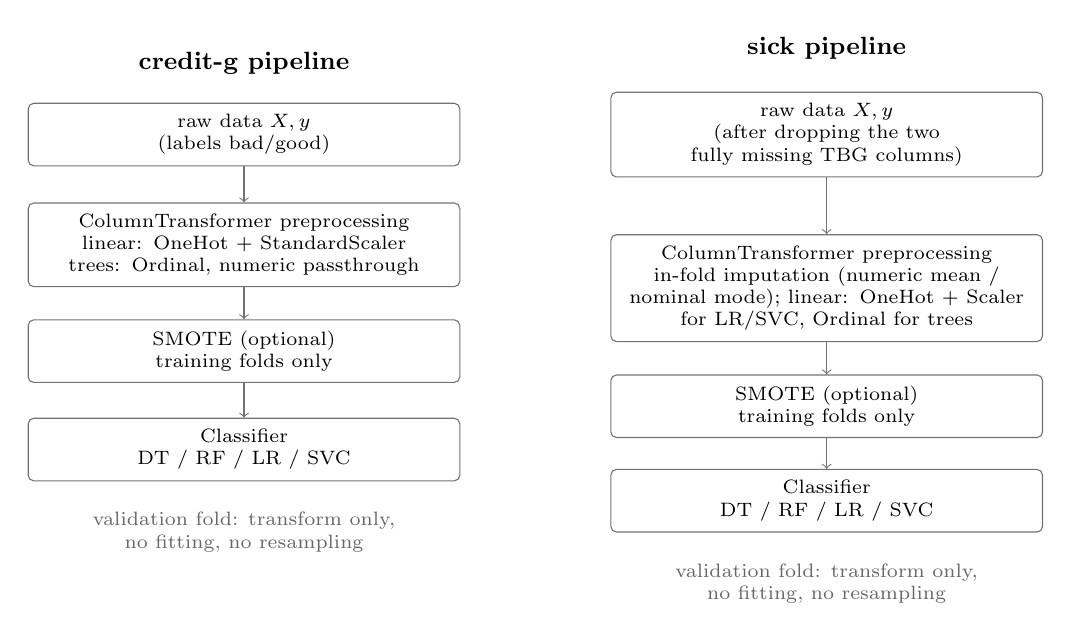
\begin{tikzpicture}[
  box/.style={draw=black!55, rounded corners=2pt, align=center,
              font=\scriptsize, text width=5.2cm, inner sep=4pt},
  ttl/.style={font=\small\bfseries},
  note/.style={font=\scriptsize, text=black!60, align=center}]
% ---- credit-g column ----
\node[ttl]        at (0,0.9)    {credit-g pipeline};
\node[box] (raw1) at (0,0)      {raw data $X,y$\\(labels bad/good)};
\node[box] (pre1) at (0,-1.4)   {ColumnTransformer preprocessing\\linear: OneHot + StandardScaler\\trees: Ordinal, numeric passthrough};
\node[box] (sm1)  at (0,-2.75)  {SMOTE (optional)\\training folds only};
\node[box] (clf1) at (0,-4.0)   {Classifier\\DT / RF / LR / SVC};
\draw[->,black!55] (raw1) -- (pre1);
\draw[->,black!55] (pre1) -- (sm1);
\draw[->,black!55] (sm1) -- (clf1);
\node[note]        at (0,-5.05) {validation fold: transform only,\\no fitting, no resampling};
% ---- sick column ----
\node[ttl]        at (7.4,1.1)  {sick pipeline};
\node[box] (raw2) at (7.4,0)    {raw data $X,y$\\(after dropping the two\\fully missing TBG columns)};
\node[box] (pre2) at (7.4,-1.95) {ColumnTransformer preprocessing\\in-fold imputation (numeric mean /\\nominal mode); linear: OneHot + Scaler\\for LR/SVC, Ordinal for trees};
\node[box] (sm2)  at (7.4,-3.45) {SMOTE (optional)\\training folds only};
\node[box] (clf2) at (7.4,-4.65) {Classifier\\DT / RF / LR / SVC};
\draw[->,black!55] (raw2) -- (pre2);
\draw[->,black!55] (pre2) -- (sm2);
\draw[->,black!55] (sm2) -- (clf2);
\node[note]        at (7.4,-5.7) {validation fold: transform only,\\no fitting, no resampling};
\end{tikzpicture}
\caption{The two dataset-specific pipelines share one three-stage
structure, from preprocessing through optional SMOTE to the
classifier. They differ only inside the preprocessing stage, where
sick additionally imputes missing values in-fold. The validation fold
is only transformed, never fitted or resampled.}
\label{fig:pipelines}
\end{figure}

\subsection{Locked Configuration}
All hyperparameters were frozen once, before any evaluation, with
\texttt{random\_state=42} on every stochastic component:
\begin{itemize}
\item DT: \texttt{criterion='entropy'}, $\alpha_{\text{ccp}}=0.01$;
\item RF: $n_{\text{estimators}}=100$;
\item LR: \textit{max\_iter}=1000, leaving convergence headroom on
the 60--80 one-hot dimensions;
\item SVC: RBF kernel, $C=1.0$, \texttt{probability=True}.
\end{itemize}
The values follow library defaults or simple round settings and were
deliberately not tuned, so no evaluation signal could leak into model
selection. Together with the locked splits and the seed they make the
pipeline reproducible. Reported numbers are checked against the
archived outputs within a tight tolerance, since floating-point
results can still differ slightly across hardware and threading
configurations.
% TODO(E): cite scikit-learn (Pedregosa et al., 2011) and
% imbalanced-learn (Lemaitre et al., 2017) once bib keys are fixed.

\subsection{Evaluation Protocol}
Two fixed protocols are used. The first is stratified 10-fold
cross-validation with \texttt{shuffle=True} and
\texttt{random\_state=42} over the full data, reported as
mean$\pm$std over folds with $ddof=0$. The second is a one-off 70:30
stratified holdout, 700/300 on credit-g and 2640/1132 on sick,
evaluated exactly once per locked configuration. Since the champion
configuration was selected on the full-data CV and those folds
overlap the holdout rows, the holdout is not an untouched final test.
We therefore report the two protocols as fixed internal evaluations
and note the selection overlap as a limitation. The minority class is
the positive class throughout, bad on credit-g and sick on sick. All
metrics come from one shared evaluation module: accuracy,
positive-class precision, recall and F1, ROC-AUC, Cohen's $\kappa$,
balanced accuracy, macro-F1, and the credit-g cost
$(5\,\mathit{FN}+\mathit{FP})/N$.

% [review note] Former subsection "Dataset-Specific Differences" (table
% tab:pipeline-diff) deleted after review: the differences it tabulated are
% already given in Sections 3a/3b and in the pipeline figure above.

% [M6, per D's v2.1 write-back note] The former "Ensemble study setup" paragraph
% now lives at the start of Section 6.5 (sec6_results.tex) and was removed here.

\renewcommand{\theHfigure}{D.\arabic{figure}}\renewcommand{\theHtable}{D.\arabic{table}}
\setcounter{section}{5}\refstepcounter{section}\setcounter{subsection}{0}\label{sec:results}\addcontentsline{toc}{section}{6 Results and Evaluation}


\section*{6 Results and Evaluation}

The main matrix compares four classifiers under plain, SMOTE, cost-sensitive and
threshold-adjusted training. Metrics refer to \texttt{bad} on credit-g and
\texttt{sick} on sick. Section 6.1 reports model selection and metric choice;
Section 6.2 tests strategy effects; Section 6.3 examines preprocessing;
Section 6.4 evaluates holdout errors; Section 6.5 adds exploratory evidence.
Data preparation and validation are defined in Sections 3 and 5.

\subsection*{6.1 Main Results across Two Datasets}

\begin{center}
\begin{minipage}{\textwidth}
\centering
{\footnotesize\textbf{Table 6.1}\ \ credit-g positive-class F1 under ten-fold CV}

\footnotesize
\begin{tabular}{p{1.35in}p{0.95in}p{0.95in}p{0.95in}p{0.95in}}
\toprule
Model & Plain & SMOTE & Cost-sensitive & Threshold \\
\midrule
Decision Tree & $0.322 \pm 0.192$ & $0.471 \pm 0.078$ & $0.523 \pm 0.030$ & $0.561 \pm 0.038$ \\
Random Forest & $0.499 \pm 0.079$ & $0.509 \pm 0.077$ & $0.595 \pm 0.064$ & $0.595 \pm 0.059$ \\
Logistic Regression & $0.531 \pm 0.060$ & $0.591 \pm 0.051$ & $\mathbf{0.597 \pm 0.034}$ & $0.591 \pm 0.049$ \\
SVC & $0.498 \pm 0.101$ & $0.560 \pm 0.050$ & $0.593 \pm 0.032$ & $0.590 \pm 0.055$ \\
\midrule
\multicolumn{5}{l}{ZeroR reference: F1 $=0$; accuracy $=0.700$; recall $=0$} \\
\bottomrule
\end{tabular}
\end{minipage}
\end{center}

\begin{center}
\begin{minipage}{\textwidth}
\centering
{\footnotesize\textbf{Table 6.2}\ \ sick positive-class F1 under ten-fold CV}

\footnotesize
\begin{tabular}{p{1.35in}p{0.95in}p{0.95in}p{0.95in}p{0.95in}}
\toprule
Model & Plain & SMOTE & Cost-sensitive & Threshold \\
\midrule
Decision Tree & $0.836 \pm 0.050$ & $0.747 \pm 0.050$ & $0.836 \pm 0.050$ & $0.820 \pm 0.048$ \\
Random Forest & $0.870 \pm 0.047$ & $\mathbf{0.897 \pm 0.051}$ & $0.873 \pm 0.048$ & $0.877 \pm 0.052$ \\
Logistic Regression & $0.687 \pm 0.091$ & $0.521 \pm 0.028$ & $0.687 \pm 0.091$ & $0.745 \pm 0.038$ \\
SVC & $0.763 \pm 0.064$ & $0.742 \pm 0.039$ & $0.763 \pm 0.064$ & $0.809 \pm 0.039$ \\
\midrule
\multicolumn{5}{l}{ZeroR reference: F1 $=0$; accuracy $=0.939$; recall $=0$} \\
\bottomrule
\end{tabular}
\end{minipage}
\end{center}

Values are means $\pm$ population SD across ten folds; bold marks the
highest mean in each main matrix. Credit-g uses 5:1 cost weights; sick uses an
equal-cost 1:1 control. Source: \texttt{results/all\_metrics\_v1.csv}.

\begin{enumerate}
\item \textbf{The best combination changes with the dataset.} Cost-weighted Logistic
Regression leads credit-g; Random Forest with SMOTE leads sick. Figure 6.1 visualises
the complete matrices, including the variability across model--strategy combinations.
\item \textbf{Minority detection requires more than accuracy.} ZeroR predicts the
majority label throughout. Its high accuracy and zero recall justify evaluating
positive-class F1, precision and recall alongside the task-specific cost.
\item \textbf{The same intervention can help or harm.} Every intervention raises
credit-g F1 relative to its own plain model. On sick, SMOTE lowers F1 for DT, LR and
SVC. For LR, recall rises from 0.606 to 0.870 but precision falls from 0.803 to 0.373:
detecting more positives does not guarantee a better F1.
\item \textbf{Ranking curves and classification errors are complementary.} The RF
curves in Figure 6.2 are similar across plain, SMOTE and equal-cost training. This is
an observation for these configurations. Threshold adjustment preserves the same
fitted scores by construction. Pooled curve statistics and fold-averaged table
metrics use different aggregation.
\end{enumerate}

\begin{center}
\begin{minipage}{\textwidth}
\centering
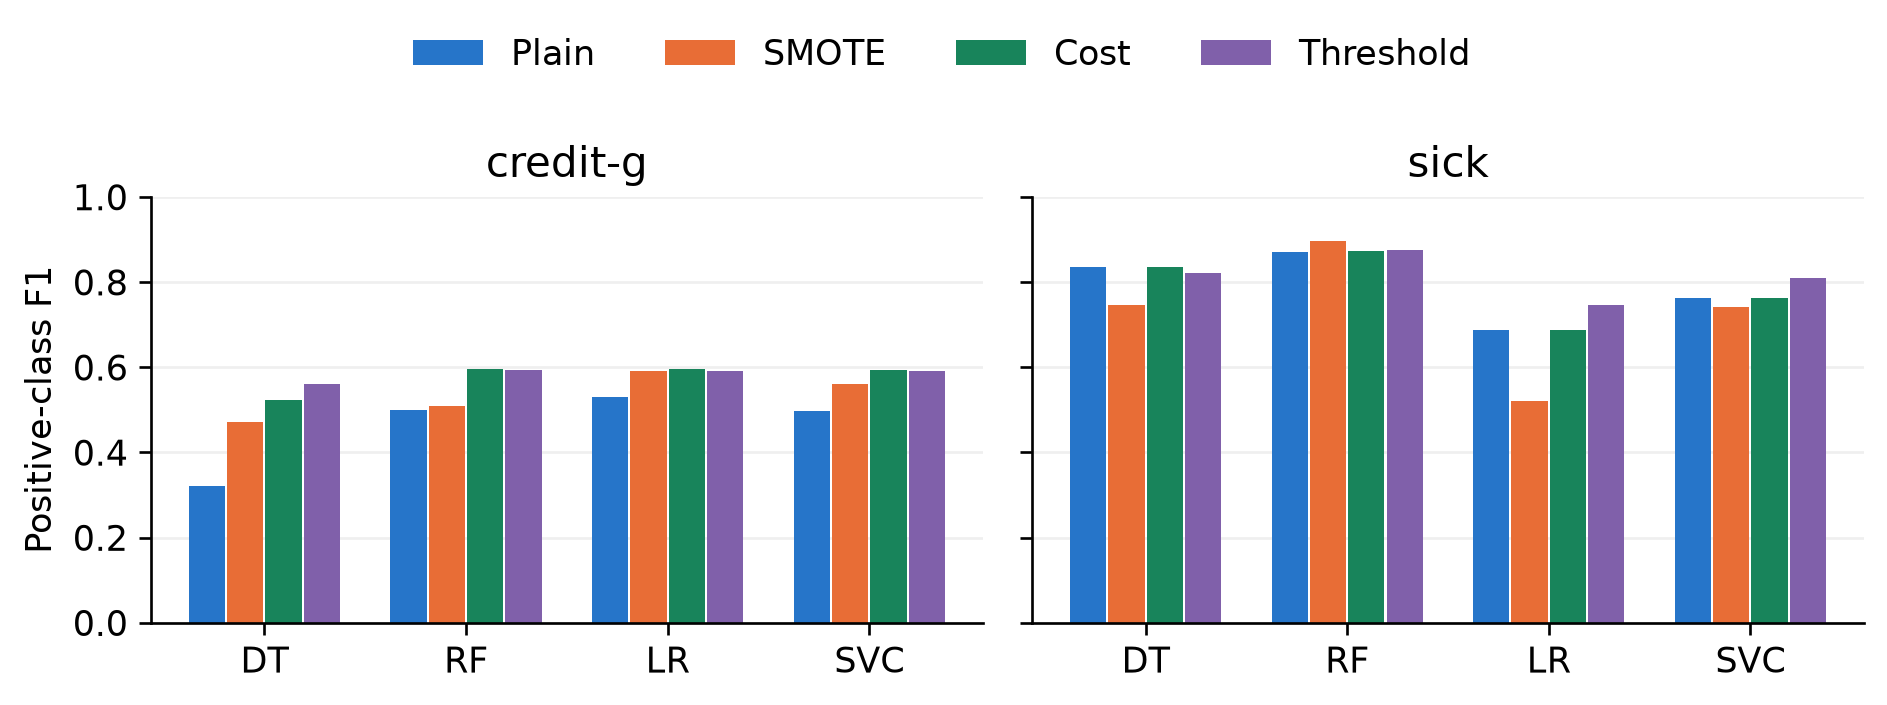
\includegraphics[width=\textwidth]{fig_6_1_main_f1.png}

{\footnotesize\textbf{Figure 6.1}\ \ Mean F1 for the complete main matrices. DT = Decision
Tree; RF = Random Forest; LR = Logistic Regression. All scores use ten-fold CV. SDs
are retained in Tables 6.1--6.2. Source: \texttt{all\_metrics\_v1.csv}.}
\end{minipage}
\end{center}

\begin{center}
\begin{minipage}{\textwidth}
\centering
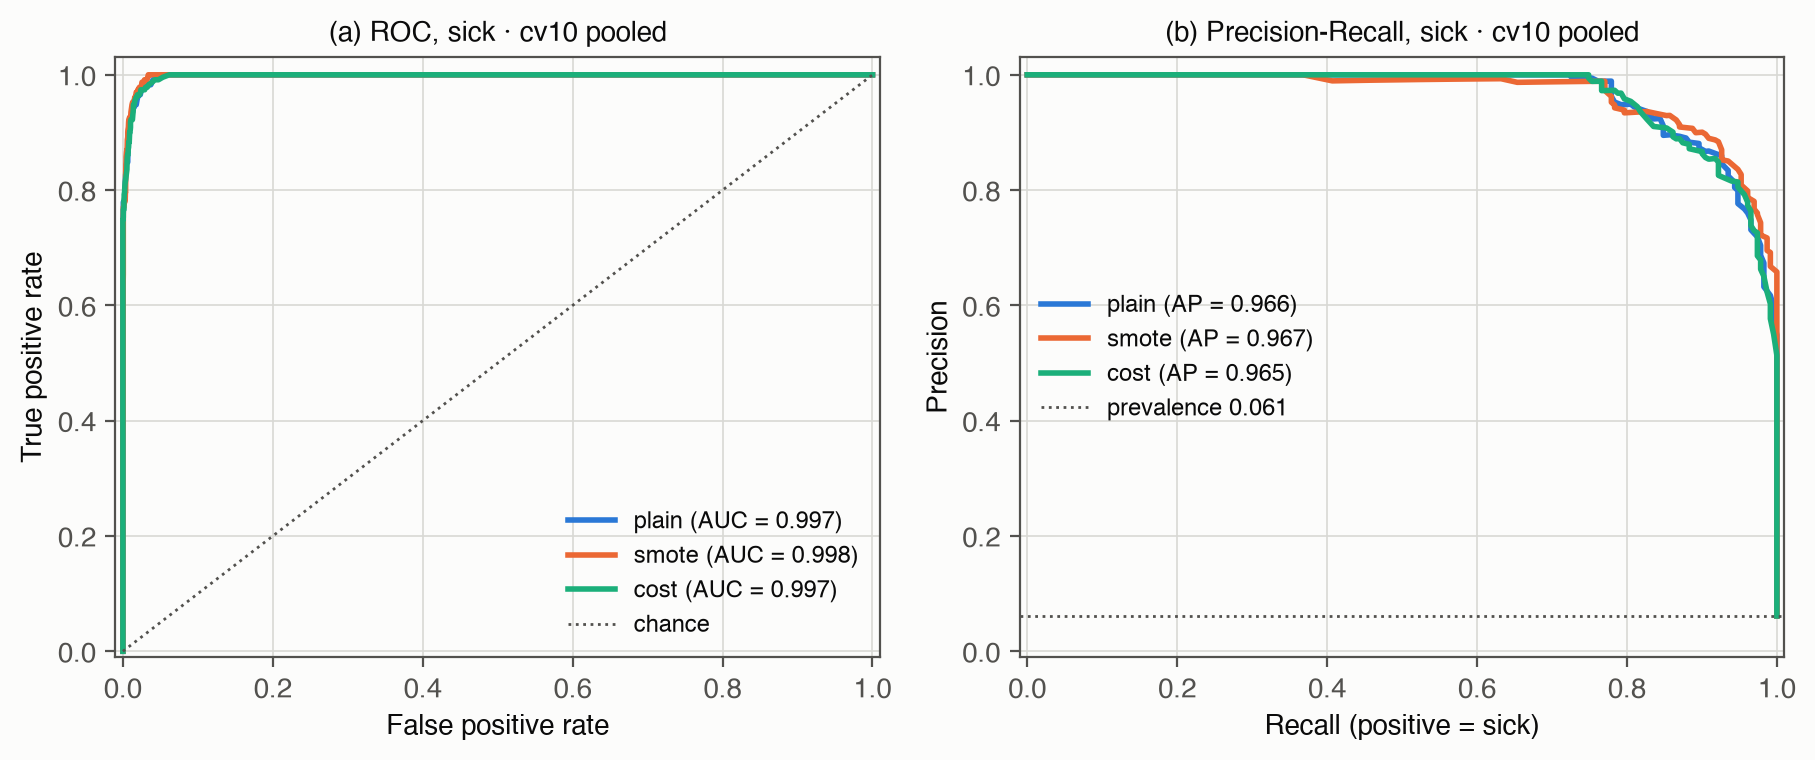
\includegraphics[width=0.88\textwidth]{fig_6_2_roc_pr.png}

{\footnotesize\textbf{Figure 6.2}\ \ RF ROC and precision--recall curves on sick. All 3,772
out-of-fold predictions are pooled; positive = sick. AP denotes average precision.
Dotted lines mark chance and prevalence. Source:
\texttt{results/preds/sick\_rf\_*\_cv10\_preds.csv}.}
\end{minipage}
\end{center}

\subsection*{6.2 Strategy Effects and Statistical Evidence}

\begin{center}
\begin{minipage}{\textwidth}
\centering
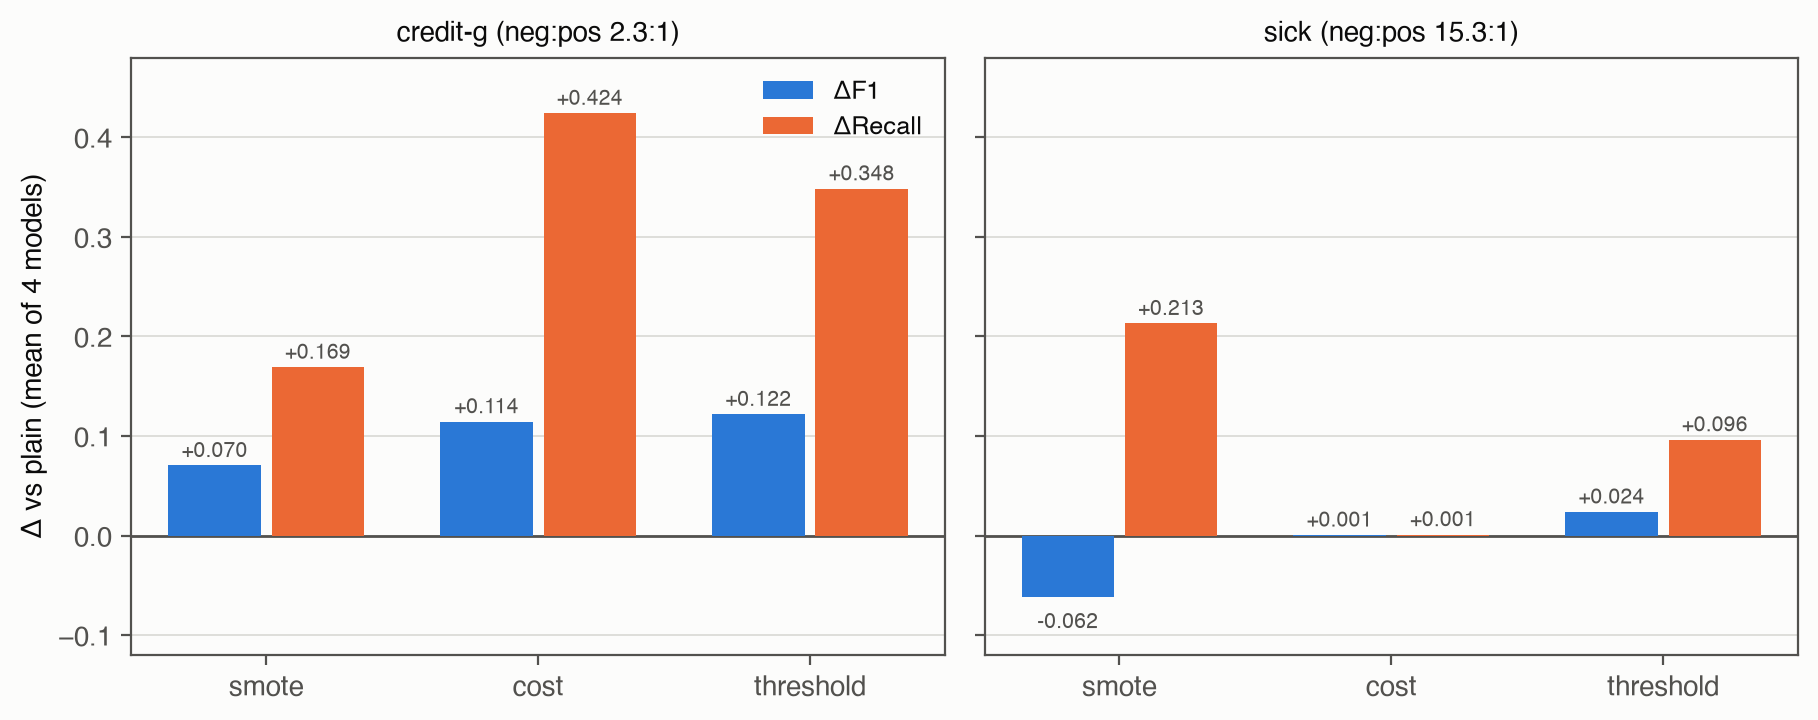
\includegraphics[width=\textwidth]{fig_6_3_strategy_gain.png}

{\footnotesize\textbf{Figure 6.3}\ \ Mean change from plain training across four classifiers,
using ten-fold CV. These are descriptive changes, not significance tests. Ratios
denote negative:positive counts. Source: \texttt{cross\_dataset\_comparison\_v1.csv}.}
\end{minipage}
\end{center}

\begin{center}
\begin{minipage}{\textwidth}
\centering
{\footnotesize\textbf{Table 6.3}\ \ Counts of significant strategy-versus-plain contrasts}

\footnotesize
\begin{tabular}{p{0.8in}p{0.75in}p{0.75in}p{0.95in}p{0.9in}}
\toprule
Dataset & Metric & Tested & Raw $p<.05$ & Holm $p<.05$ \\
\midrule
credit-g & F1 & 12 & 3 & 0 \\
sick & F1 & 12 & 2 & 0 \\
credit-g & Recall & 12 & 11 & 8 \\
sick & Recall & 12 & 7 & 2 \\
\bottomrule
\end{tabular}
\end{minipage}
\end{center}

Following the corrected paired-test procedure of Section 5, Nadeau--Bengio corrected
paired $t$-tests account for the overlap of training folds, and the Holm adjustment is
applied over all 120 pairwise contrasts among the 16 configurations, separately for
each dataset and metric; Table 6.3 reports the twelve pre-specified within-model
strategy contrasts from each family. Source: \texttt{results/ttest/}.

\begin{enumerate}
\item \textbf{Recall has stronger statistical support.} Across both datasets, recall
increases in 21 contrasts and is unchanged in three. Ten of 24 recall contrasts
survive Holm correction; none of the 24 F1 contrasts does. The highest observed F1 is
therefore a selection criterion, not proof of significant superiority.
\item \textbf{Averaging hides important exceptions.} Figure 6.3 summarises the overall
pattern. Table 6.2 identifies four sick F1 losses: SMOTE with DT, LR and SVC, and
threshold adjustment with DT. Model-specific results remain necessary when selecting
a strategy.
\item \textbf{Non-significance is not equivalence.} The conservative correction limits
claims about improvements; it does not establish that configurations perform equally.
Recall, precision and the error-cost objective should be considered together.
\end{enumerate}

\subsection*{6.3 Cross-Dataset Comparison and Preprocessing Evidence}

\begin{center}
\begin{minipage}{\textwidth}
\centering
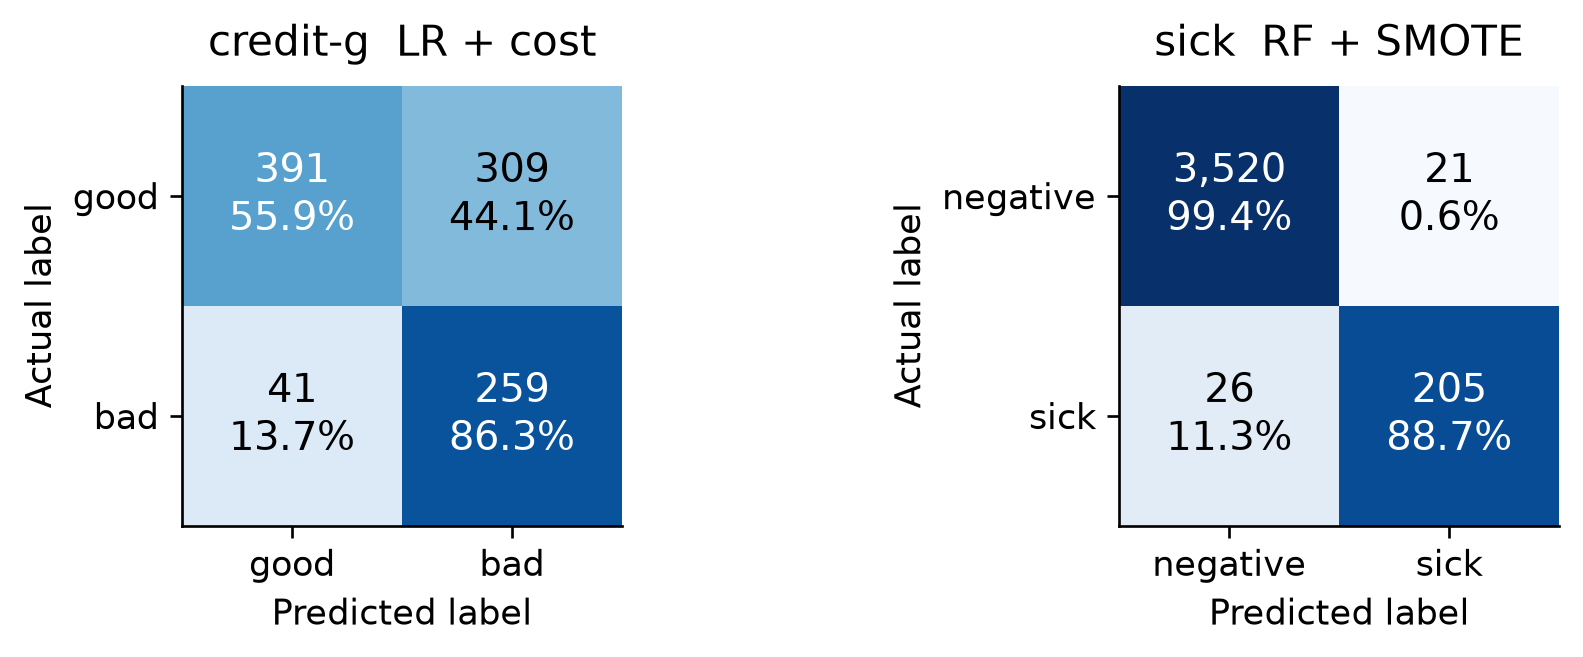
\includegraphics[width=\textwidth]{fig_6_4_confusion.png}

{\footnotesize\textbf{Figure 6.4}\ \ Main-matrix winners, pooled ten-fold CV. Each cell gives
count and percentage within its actual class. Rows = actual; columns = predicted.
Positive labels: \texttt{bad} and \texttt{sick}. Source: \texttt{all\_metrics\_v1.csv}.}
\end{minipage}
\end{center}

\begin{enumerate}
\item \textbf{The selected models carry different error burdens.} In Figure 6.4 the
credit-g champion identifies 86.3\% of bad records but flags 44.1\% of good ones;
the sick champion identifies 88.7\% of positives with only 0.6\% false alarms among
negatives (counts in Figure 6.4). Both winners were selected by F1, yet their error
profiles differ sharply; Section 6.4 evaluates the decision trade-offs of both
configurations. The simultaneous differences in size, attributes, missingness and
imbalance (Section 3) prevent isolating a single cause.
\item \textbf{Encoding evidence supports a specific LR choice.} Credit-g LR gives F1
0.531 with one-hot, 0.406 with ordinal and 0.415 with standardised ordinal encoding.
This supports the tested LR pipeline. Categorical interpolation is a hypothesis for
SMOTE losses.
\item \textbf{Missing-data handling trades retention against performance.} For
Decision Tree on sick under stratified ten-fold CV: fold-internal imputation scores
F1 $0.830 \pm 0.049$ with AUC $0.974$; dropping the 1,129 incomplete records ---
19 of the 231 positives among them --- scores $0.843 \pm 0.069$ with AUC $0.964$;
treating ``missing'' as its own category scores F1 0.828 with AUC 0.965. Deletion
nominally leads on F1 but sits within one standard deviation of imputation while
discarding those records; imputation preserves every positive and posts the best AUC.
Decision: impute inside the pipeline. Overlapping spreads and changed samples
preclude a stricter equivalence claim. Source:
\texttt{results/b4\_missing\_comparison.csv}.
\end{enumerate}

\subsection*{6.4 Holdout Results and Decision Trade-offs}

\begin{center}
\begin{minipage}{\textwidth}
\centering
{\footnotesize\textbf{Table 6.4}\ \ Main-matrix winners on the fixed 70:30 holdout}

\footnotesize
\begin{tabular}{p{0.75in}p{1.15in}p{0.9in}p{0.65in}p{0.8in}p{0.55in}p{0.55in}}
\toprule
Dataset & Configuration & N / positive & Recall & Precision & F1 & Cost \\
\midrule
credit-g & LR + cost & 300 / 90 & 0.822 & 0.448 & 0.580 & 0.570 \\
sick & RF + SMOTE & 1,132 / 69 & 0.957 & 0.868 & 0.910 & --- \\
\bottomrule
\end{tabular}
\end{minipage}
\end{center}

Credit-g cost follows Section 5; sick has no official cost matrix.
Source: holdout rows of \texttt{all\_metrics\_v1.csv}.

\begin{enumerate}
\item \textbf{Decisions have measurable trade-offs.} Credit-g LR + cost misses 16
bad-labelled records and flags 91 good-labelled records. Cost falls to 0.570 from
0.887 for plain LR and 1.500 for ZeroR. RF + threshold has lower cost at 0.543, so F1
selection is not cost minimisation. Sick RF + SMOTE produces three misses and ten
false alarms.
\item \textbf{Holdout is an internal assessment.} Full-data CV informed selection; the
overlapping holdout is not an independent final test. These historical benchmarks do
not establish deployment readiness.
\end{enumerate}

\subsection*{6.5 Exploratory Ensembles and Association Rules}

\begin{center}
\begin{minipage}{\textwidth}
\centering
{\footnotesize\textbf{Table 6.5}\ \ Complete exploratory ensemble results under ten-fold CV}

\footnotesize
\begin{tabular}{p{0.75in}p{1.3in}p{1.05in}p{0.65in}p{0.55in}p{0.55in}}
\toprule
Dataset & Configuration & $\text{F1 mean} \pm \text{SD}$ & Recall & AUC & Time s \\
\midrule
credit-g & Bagging + plain & $0.510 \pm 0.072$ & 0.430 & 0.782 & 2.2 \\
credit-g & Bagging + SMOTE & $\mathbf{0.548 \pm 0.074}$ & 0.560 & 0.770 & 1.2 \\
credit-g & AdaBoost + plain & $0.499 \pm 0.070$ & 0.473 & 0.735 & 1.2 \\
credit-g & AdaBoost + SMOTE & $0.501 \pm 0.087$ & 0.483 & 0.723 & 2.4 \\
sick & Bagging + plain & $0.819 \pm 0.050$ & 0.775 & 0.990 & 3.6 \\
sick & Bagging + SMOTE & $0.785 \pm 0.037$ & 0.987 & 0.994 & 4.6 \\
sick & AdaBoost + plain & $0.918 \pm 0.045$ & 0.901 & 0.999 & 9.5 \\
sick & AdaBoost + SMOTE & $\mathbf{0.937 \pm 0.043}$ & 0.931 & 0.999 & 28.9 \\
\bottomrule
\end{tabular}
\end{minipage}
\end{center}

Bold marks each dataset's highest exploratory mean. Time is recorded
fitting time. These configurations are outside the main statistical family. Source:
\texttt{ensemble\_metrics\_v1.csv}.

\begin{enumerate}
\item \textbf{High recall does not guarantee a better balance.} On sick, Bagging +
SMOTE pushes recall to 0.987 while F1 falls to 0.785 (plain 0.819); AdaBoost + SMOTE
instead keeps recall at 0.931 with F1 0.937, the highest exploratory mean, though its
gap to the main-matrix winner RF + SMOTE (0.897) was not tested. Among the four
exploratory tests outside the main Holm family, only sick AdaBoost plain versus DT +
SMOTE meets the raw threshold ($p = 0.000639$). The precision--recall trade-off
depends on the model, even under the same resampling strategy.
\item \textbf{Rules add a different interpretation.} The highest-duration bin with
savings below 100 covers 124 records, including 71 bad labels: confidence 0.573 and
lift 1.91. Six rules meet confidence $\geq 0.50$ and a five-percentage-point gain over
the stronger single-condition rule. Some fields recur in tree interpretations, but no
complete selected rule is reproduced. Apriori uses all 1,000 records; the trees use
700 training records. Their overlap is complementary interpretation, not independent
validation.
\end{enumerate}


\subsection*{6.6 Association Rule Evidence}
\phantomsection\makeatletter\def\@currentlabel{6.6}\makeatother
\paragraph{Association rule evidence.}\label{sec:apriori} Apriori found simple combinations associated with the bad label and added to the supervised model explanations. The leading rule combined the highest duration band with savings below 100. Among 124 matching records, 71 were labelled bad. Support was 0.071, confidence 0.573 and lift 1.91, compared with an overall bad proportion of 0.30. We retained six rules with confidence of at least 0.50 and a gain of at least five percentage points over the stronger single condition. We discretised three continuous fields, then mined frequent itemsets from 1,000 Boolean transactions using minimum support 0.05 and at most three items per itemset. Some fields also appeared in decision tree paths and ranked highly in random forest importance, but the tree reproduced no complete selected rule. This overlap helps interpretation, but does not independently validate the rules. The rules were selected using all records and establish neither causation nor predictive accuracy.

\setcounter{section}{6}\refstepcounter{section}\addcontentsline{toc}{section}{7 Conclusion and Future Work}
\section*{7 Conclusion and Future Work}

\subsection*{7.1 Findings}

\begin{enumerate}
\item \textbf{(RQ1) Selection depends on the dataset.} Cost-weighted LR leads the
credit-g main matrix at F1 0.597; RF + SMOTE leads sick at 0.897. Section 6.2 supports
recall gains more strongly than F1 gains. No intervention improves every model on both
datasets.
\item \textbf{(RQ2) Accuracy needs minority-class evidence.} The reference rows in
Tables 6.1--6.2 illustrate the limitation of accuracy. Positive-class precision, recall
and F1, together with relevant error costs, reveal the decision trade-offs.
\item \textbf{(RQ3) One-hot encoding favours the tested LR pipeline; imputation
preserves sick records.} One-hot reaches F1 0.531 against 0.406 with ordinal codes on
credit-g LR; imputation retains all 3{,}772 sick records with the best AUC among the
three tested missing-data schemes (0.974). These conclusions are scoped to the tested
configurations; dataset differences and shared explanatory fields do not establish
causal mechanisms.
\item \textbf{(RQ4) The champions cut holdout cost and missed positives.} On the
holdout, credit-g cost falls to 0.570 from 0.887 for plain LR and 1.500 for
always-approve ZeroR, and the sick champion misses 3 of 69 positives with ten false
alarms. Section 6.4 bounds these results to internal evaluation because model
selection and final testing were not fully independent.
\end{enumerate}


\subsection*{7.2 Limitations}
These results describe internal comparisons on two datasets using one split seed. They do not establish performance on new populations. Retained duplicate sick records may appear in different validation folds. Configuration selection used cross validation over all records, so the overlapping holdout does not provide an independent test of that selection. Ordinary SMOTE can create artificial categorical representations, but we did not isolate their effect on performance. The ensemble extension and Apriori analysis are exploratory. We did not directly test the higher ensemble F1 against the main experiment winner. These limits leave uncertainty about generalisation and the reasons for model differences.

\subsection*{7.3 Future Work}
The next step is to test the selected configurations on independent data, or use nested cross validation with several seeds. A controlled comparison with SMOTENC could test whether preserving categorical values improves resampling. Threshold selection should follow the decision objective, including the official credit cost matrix where applicable. The Apriori rules also need checks on separate samples to see whether their support, confidence and lift remain stable.



% Bibliography (if required)
\bibliographystyle{plain}
\bibliography{references}

\clearpage
\section*{Team Contributions}
\label{sec:contributions}

Table~\ref{tab:contributions} records each member's role and specific work. All five members reviewed and confirmed the approximate workload shares shown below.

\begin{table}[htbp]
\centering
\small
\caption{Individual contributions and approximate workload shares. Shares total 100\%.}
\label{tab:contributions}
\begin{tabular}{@{}p{0.18\linewidth}p{0.16\linewidth}p{0.50\linewidth}p{0.09\linewidth}@{}}
\toprule
Member (ID) & Role & Specific contribution & Share \\
\midrule
HU Zhongyuan (3162304) & Dataset A owner & credit-g source, schema, quality audit and preprocessing; credit-g ensemble runs; Introduction and credit-g sections & 20\% \\
LING Tong (3162677) & Dataset B owner & sick source, labels, missingness audit and preprocessing; sick ensemble runs; sick section and data-quality figures & 20\% \\
CHEN Yanwu (3162744) & Modeling lead & Reproducible Python pipelines, classifier and strategy runs, ensemble setup and statistical tests; methods sections and demonstration & 20\% \\
CHEN Yinan (3162550) & Evaluation and visualization lead & Evaluation protocol, metrics and statistical comparison; results tables, figures, cross-dataset analysis and conclusions & 20\% \\
ZHANG Yijie (3162641) & Writing and coordination lead & Apriori preparation, rules and tree comparison; report structure, references, contribution appendix, integration and presentation coordination & 20\% \\
\bottomrule
\end{tabular}
\end{table}



\end{document}
